\chapter{Atom number estimation for Clock-state atoms surrounding a nanofiber}
In the case that a nanofiber dispersively coupled to an atomic ensemble, if we ignore tensor 
polarizability contributions, the Hamiltonian can be rewritten as below using the Stokes operators, $ 
\hat{S}_q $, and collective spin operators, $ \hat{J}_q $, with $ q=0,1,2,3 $:
\begin{align}
H_{\rm eff} 
=\frac{\hbar}{\tau} \Big\{ & \left[ \big( \chi_{H,\uparrow} + \chi_{H,\downarrow}\big) + \big(\chi_{V,\uparrow} + \chi_{V,\downarrow}\big) \right] \hat{J}_0 \hat{S}_0 \nonumber \\
+ & \left[ \big( \chi_{H, \uparrow} + \chi_{H,\downarrow}\big) - \big( \chi_{V,\uparrow} + \chi_{V,\downarrow} \big)\right]  \hat{J}_0 \hat{S}_1 \nonumber \\
+ & \left[ \big( \chi_{H,\uparrow} - \chi_{H,\downarrow}\big) + \big(\chi_{V,\uparrow} - \chi_{V,\downarrow} \big) \right] \hat{J}_3 \hat{S}_0 \nonumber \\
+ & \left[ \big( \chi_{H,\uparrow} - \chi_{H,\downarrow}\big) - \big(\chi_{V,\uparrow} - \chi_{V,\downarrow} \big) \right]  \hat{J}_3 \hat{S}_1\Big\}.\label{eq:JScoupling}
\end{align}
Here, we assume the detuning of the optical field is much larger than the natural linewidth of the 
coupled atoms so that we can ignore the tensor contribution of the atomic polarizability. We have also 
restricted the atomic ground state within the $ 6S_{1/2} $ $ F=3 $ ($ \ket{\downarrow} $) and $ F=4 $ ($ 
\ket{\uparrow} $) clock state space\index{state!clock state} which rules out the vector contribution of 
the atomic polarizability. Therefore, we are only considering the scalar polarizability effect of the atoms 
for this problem. Effectively, the ground states span into a psuedo-spin space\index{psuedo spin}, and 
can be used for QIP with the manipulation of light. 

As has been discussed in the 2010 nanofiber proposal, if we want to estimate the state of the collective 
spins, we need to estimate the number of atoms sitting in the $ \ket{\uparrow} $ and $ \ket{\downarrow} 
$ states employing a dispersive QND measurement technique which has been well developed for the 
free-space atomic ensembles. For our system, the forth term of the Hamiltonian in 
Equ.~\eqref{eq:JScoupling} empowers us the possibility of measuring the atomic states without 
destroying them with an $ \hat{S}_3=\frac{1}{2i}(\hat{a}_H^\dagger\hat{a}_V - 
\hat{a}_V^\dagger\hat{a}_H) $ homodyne measurement. Yet, the third term of the Hamiltonian becomes 
a noisy term that brings in photon number noise into the measurement result. In the early proposal, we 
thought there is a magic wavelength for the probe light which allows us totally remove the third term. 
In the following sections, we will see that this magic wavelength does not exist for our quantum state 
estimation purpose with only scalar polarizability considered. We will also see that a two-color probe 
setup might be useful to 
achieve the goal of the high-resolution atom number measurement, the sensitivity of which has been 
experimentally demonstrated~\cite{Beguin2014}. An approach to calculating the squeezing parameters 
will also be discussed. A more general way to calculate the coupling strengths and magic frequencies 
will be given in the end of this chapter.

\section{Magic wavelength does not exist with merely scalar polarizability using a simple strategy}
From the definition of the coupling strength of various $ \chi $'s (Equs.~\eqref{chiHUp} through~\eqref{eq:AeffV}), one can show that, for $ D_1 $ line, 
\begin{align}
\chi_H \equiv \chi_{H,\uparrow} - \chi_{H,\downarrow} &= \frac{1}{3}\sum_{F'} \left(\frac{\sigma_0}{A_{\rm eff}^H} \right) \left(\frac{\Gamma}{4\Delta_{4F'}} - \frac{\Gamma}{4\Delta_{3F'}} \right) \nonumber\\
&= \frac{\Gamma_H}{3} \left(\frac{1}{\Delta_{43}}+\frac{1}{\Delta_{44}} - \frac{1}{\Delta_{33}}-\frac{1}{\Delta_{34}} \right) = \frac{\Gamma_H}{3}\Delta_-,\label{eq:chiH}\\
\chi_V \equiv \chi_{V,\uparrow} - \chi_{V,\downarrow} &= \frac{1}{3}\sum_{F'} \left(\frac{\sigma_0}{A_{\rm eff}^V} \right) \left(\frac{\Gamma}{4\Delta_{4F'}} - \frac{\Gamma}{4\Delta_{3F'}} \right) \nonumber\\
&= \frac{\Gamma_V}{3} \left(\frac{1}{\Delta_{43}}+\frac{1}{\Delta_{44}} - \frac{1}{\Delta_{33}}-\frac{1}{\Delta_{34}} \right)=\frac{\Gamma_V}{3}\Delta_-,\label{eq:chiV}
\end{align}
where $ \Delta_{FF'} $ is the detuning relative to the $ F\leftrightarrow F' $ transition gap, and $ \Delta_- = \left(\frac{1}{\Delta_{43}}+\frac{1}{\Delta_{44}} - \frac{1}{\Delta_{33}}-\frac{1}{\Delta_{34}} \right) $ is a common factor existing in both $ \chi_H $ and $ \chi_V $ quantities. $ \Gamma_H $ ($ \Gamma_V $) is the decay rate coupled to the forward propagating $ H $ ($ V $) mode of the nanofiber. 

To find the "\textit{magic wavelength}", we need to make the coupling strength factor of the third term of the Hamiltonian in Equ.~\eqref{eq:JScoupling} equal to zero. That is to say,
\begin{align}
\chi_H+\chi_V=\frac{1}{3}\left(\Gamma_H + \Gamma_V \right)\Delta_- = 0.
\end{align}
We can see that $ \frac{1}{3}\left(\Gamma_H + \Gamma_V \right) $ is always positive and does not 
depending on wavelength. Therefore, we have to let $ \Delta_-=0 $ to find the "\textit{magic 
wavelength}"\index{magic wavelength}. From the definition of $ \chi_H $ and $ \chi_V $ 
(Equs.~\eqref{eq:chiH} and~\eqref{eq:chiV}) and the Hamiltonian (Equ.~\eqref{eq:JScoupling}), we can 
find that $ \chi_H=\chi_V=0 $ and the forth term of the Hamiltonian, which is what we want to keep, also 
becomes zero. Hence, via identifying a magic wavelength and to remove the photon flux noise in the 
measurement is invalid for our initial design. Maybe we can say, the \textit{magic wavelength} does not 
exist for one-color probe configuration and by only considering scalar polarizability effects. 

This analytical conclusion has been numerically verified. 

\section{Calculating coupling strength and squeezing parameters}
Now, let us suppose we can overcome all technical difficulties and generate a spin squeezed state (SSS) based on the forth term of the Hamiltonian through an $ \hat{S}_3 $ homodyne measurement. The effective Hamiltonian becomes
\begin{align}
	H_{\rm eff} = \frac{\hbar}{\tau} \chi_{\rm eff} \hat{J}_3 \hat{S}_1
\end{align}
where $\chi_{\rm eff} = \chi_{H} - \chi_{V}=\frac{\Gamma_H-\Gamma_V}{3}\Delta_-$. As has been proved, the squeezing parameter $ \xi =\frac{\chi_{\rm eff}^2 }{4}N_LN_A $. Therefore, to calculate the squeezing parameter, we need to calculate the decay rates coupled into the $ H $ and $ V $ modes. 

Since we can treat the atomic polarizability as a scalar for our dispersive case, we have 
\begin{align}
\Gamma_H &= 2\pi \sum_g \frac{|\mathbf{u}_H(\br')\cdot \mathbf{d}_{eg}|^2}{\hbar}\left(\frac{\omega_0}{v_g} \right) \\
&\propto \sum_g \tr \left[(\mathbf{d}_{eg}^*\mathbf{d}_{eg})\cdot \mathrm{Im} [\mathbf{G}_H^*(\br',\br')] \right]  = \sum_F \tr \left[ \alpha_F \eye\cdot \mathrm{Im} [\mathbf{G}_H^*(\br',\br')]  \right],
\end{align}
where the atomic polarizability for the ground state $ F $ is defined as $ \alpha_F=\alpha_0(\Delta_{FF'})C_{J'F}^{(0)} $ is a scalar constant for the clock state. Using the emission surface technique we have learned, the equivalent dipole momentum is pointed along $ [1,1,1]/\sqrt{3} $ direction on the principle emission coordinate induced by the fiber $ H $-mode field. Since the $ H $ mode only has $ r\!_\perp $ and $ z $ components, the field only couples to the corresponding two dipole orientations with a normalization factor $ 1/3 $ for the $ D_1 $ line transitions. Similar conclusion goes to the $ \Gamma_V $ calculation. One can also consider this problem in the perspective of quantum jumps. Since all quantum transitions ($ \pi\rm{ and }\sigma_\pm $) have the same possibility ($C_{J'FF'}^{(0)}=C_{J'F}^{(0)}=1/3 $), the decay rate is only determined by the non-zero field components with corresponding quantum transition probability. The final result does not depend on how we define the quantization axis while the details of calculation might be. 

\textcolor{blue}{Aside note: the atomic polarizability tensor is positive semidefinite, which indicates the controllability of the photon modes via controlling the atomic state. Our formalism enable us to treat this system as a linear system for controlling light with atom or vice verse. I will make a note on controllability and observability of the system, if I got a chance. I would also like to take a deeper look into the active and autonomous control theory (with error correction) of the open photonic system once time permits. Some results in quantum tomography as a branch of optimization theory may also be able to applied to the control problem, IMHO. }

With the knowledge of the equivalent dipole orientation, we can easily calculate the corresponding decay rates goes into the forwarding $ H $ and $ V $ modes respectively using any of the equivalent techniques we have learned. Plots below (Figs.~\ref{fig:HVdecayrates} and~\ref{fig:squeezingparaTerms}) illustrate the decay rates and $ \xi/N_LN_A $ as functions of frequency and atom positions relative to the fiber axis. Notice that, we have assumed that the decay rate is a constant within the small detuning around $ D_1 $ line transition frequency, which should be valid. 

\begin{figure}
\begin{minipage}{.91\linewidth}
\centering
{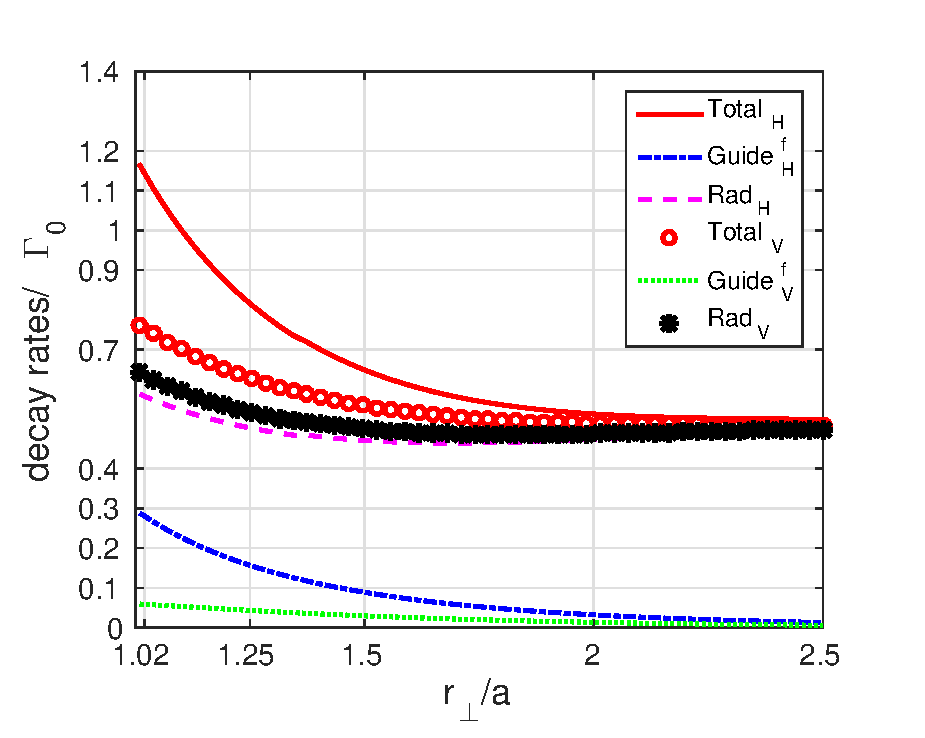
\includegraphics[scale=0.75]{../media/Figs/HVdecayrates}}
\end{minipage}
\caption{Decay rates coupled to the $ H $ and $ V $ nanofiber modes. For the guided mode contributions, only the forward propagating mode contributions are plotted out. The total decay rates for the two mode contributions have both backward and forward propagating components counted.}\label{fig:HVdecayrates}
\end{figure}

\begin{figure}
\begin{minipage}{.91\linewidth}
\centering
\subfloat[]{\label{squeezingparaTerm3}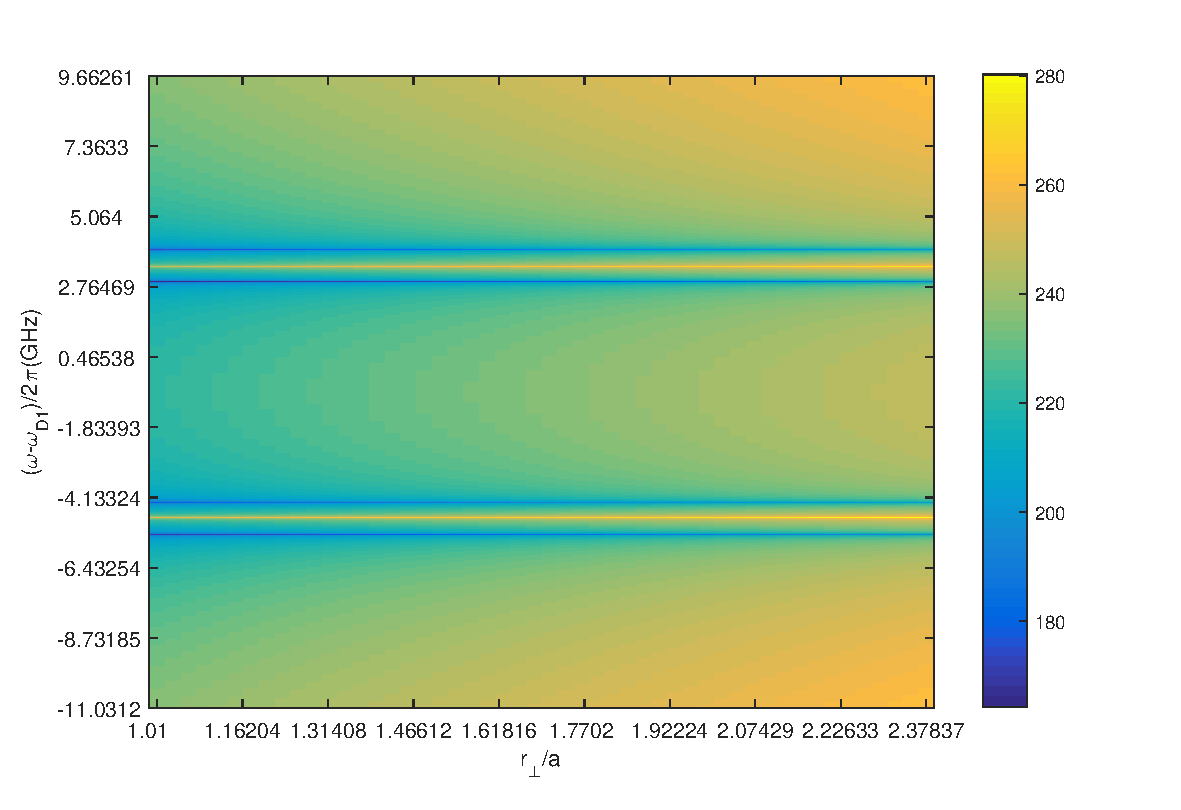
\includegraphics[scale=0.55]{../media/Figs/squeezingparaTerm3}}
\end{minipage}
\par\medskip
\begin{minipage}{.91\linewidth}
\centering
\subfloat[]{\label{squeezingparaTerm4}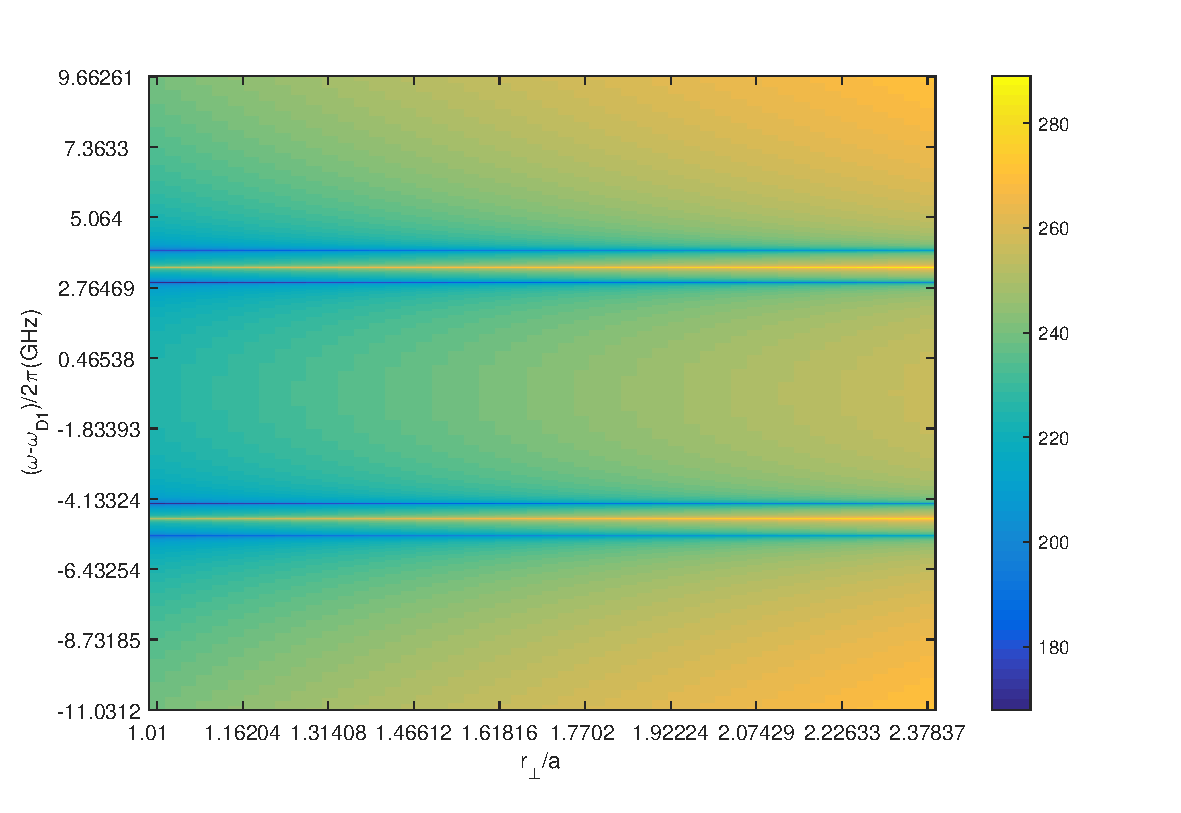
\includegraphics[scale=0.55]{../media/Figs/squeezingparaTerm4}}
\end{minipage}
\caption{Squeezing parameters associated to the third and forth terms of the Hamiltonian. The colormap shows the value of $ -10\log_{10}(\xi/N_LN_A) $. }
\label{fig:squeezingparaTerms}
\end{figure}

\begin{figure}
\begin{minipage}{.91\linewidth}
\centering
{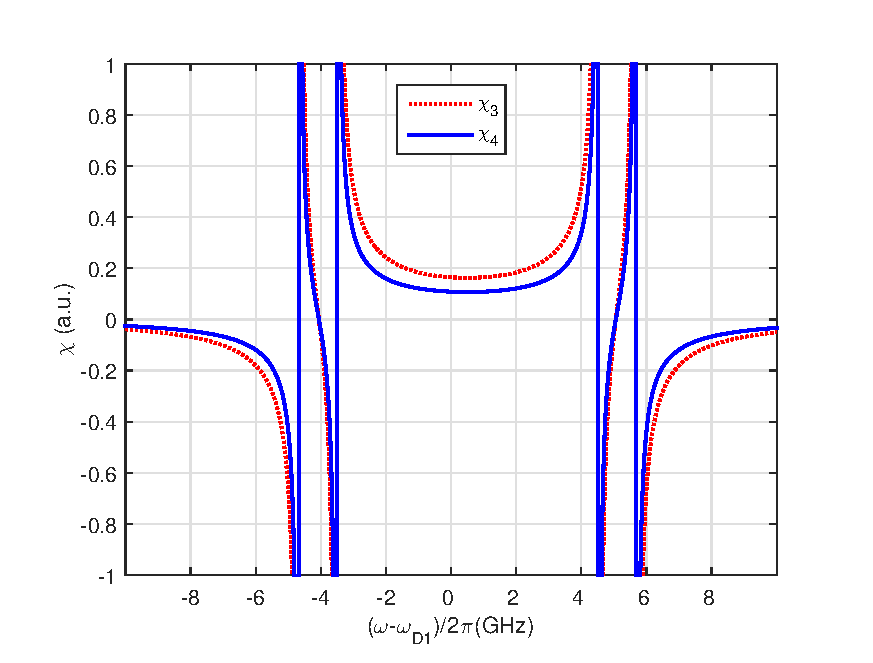
\includegraphics[scale=0.75]{../media/Figs/chi34}}
\end{minipage}
\caption{The coupling strengths for the third ($ \chi_3 $) and forth ($ \chi_4 $) terms of the Hamiltonian expressed in Equ.~\eqref{eq:JScoupling} for the $ D_1 $ line transitions associated with the clock states.} \label{fig:chi34}
\end{figure}

As shown in Fig.~\ref{fig:chi34} regarding the coupling strengths of the third and forth terms of the one-color probe Hamiltonian, the two peaks on the negative frequency side and those on the positive frequency side correspond to the approximate frequencies one can use to detect the $ \ket{\uparrow} $ and $ \ket{\downarrow} $ atom numbers. The two Hamiltonian terms seems very close to each other due to the small $ \Gamma_V $. How large will the photon fluctuation affect the final result is not clear. 

\newpage

\section{Estimate psuedo-spin state and atom number in a high resolution}
Now we come to the question "is there any way to remove the photon fluctuation from the homodyne measurement?" One way that might work is to use two-probe light signals to commit the measurement. The basic idea follows. 

If we use two-color probes for each measurement configuration, it might be possible to find non-trivial magic wavelengths to cancel the third term of the Hamiltonian. The key is that, for two distinguishable colors, the decay rates coupled to the corresponding guided modes are distinguishable as well, which may result in magic wavelengths that does not totally remove the coupling strengths at the same time. For instance, if we choose the two probes around $ D_1 $ and $ D_2 $ transition frequencies at $ \omega_1 $ and $ \omega_2 $, the two sets of $ \Gamma_{H/V}(\omega_1) $ and $ \Gamma_{H/V}(\omega_2) $ will be different. Quantitatively, the third term of the effective Hamiltonian can now be given by
\begin{align}
\!\!\!\!\!\!\!\!\!\!\hat{H}_{\rm eff}^3(\omega_1,\omega_2) &= \frac{\hbar}{\tau} \left[\chi_H(\omega_1)+\chi_H(\omega_2) + \chi_V(\omega_1)+\chi_V(\omega_2) \right] \hat{J}_3\hat{S}_0\\
&= \frac{\hbar}{3\tau} \left[  \left( \Gamma_H(\omega_1)\!+\!\Gamma_V(\omega_1) \right)\Delta_-^1(\omega_1) \!+\! 2\left( \Gamma_H(\omega_2)\!+\!\Gamma_V(\omega_2) \right)\Delta_-^2(\omega_2) \right] ,
\end{align}
where $ \Delta_-^{1/2} $ are the detuning terms due to the two colors of the probes. Similarly, the forth term of the Hamiltonian can now be given by
\begin{align}
\!\!\!\!\!\!\!\!\!\!\hat{H}_{\rm eff}^4(\omega_1,\omega_2) &= \frac{\hbar}{\tau} \left[\chi_H(\omega_1)+\chi_H(\omega_2) - \chi_V(\omega_1)-\chi_V(\omega_2) \right] \hat{J}_3\hat{S}_0\\
&= \frac{\hbar}{3\tau} \left[  \left( \Gamma_H(\omega_1)\!-\!\Gamma_V(\omega_1) \right)\Delta_-^1(\omega_1) \!+\! 2\left( \Gamma_H(\omega_2)\!-\!\Gamma_V(\omega_2) \right)\Delta_-^2(\omega_2) \right] .
\end{align}
Now that, the magic wavelengths canceling the third term of the Hamiltonian may not result in a zero coupling strength for the forth term of the Hamiltonian due to the inseparability of decay rates and detuning factors. Using differential speed of group velocity may be the key for the QUANTOP group in Denmark to success along this line~\cite{Beguin2014}. 

\textcolor{blue}{Initially, I thought we might be able to use two colors both close to the $ D_1 $ line, but 
the difference of the dispersive responses may be too small to be detected. Also, I did not consider the 
tensor and vector polarizabilities for a more general case, which may have some difference. I would also 
think more about the quantum correlation theory for our system. }

\section{Magic wavelength exists by including tensor polarizability effect}
Now, if we include the tensor polarizability effect into the Hamiltonian, and use the $ x $-axis as the 
quantization axis, the Hamiltonian can still be given in the form of Equ.~\ref{eq:JScoupling} yet with a 
different definition of the coupling strengths:
\begin{align}
\chi_{H,\uparrow/\downarrow} & \equiv \chi_{H,F} =- \frac{2\pi \omega_0}{v_g} \bra{F,0} 
	\mathbf{u}^*_H(r^\prime\!_\perp, \phi') \cdot \tensor{\alpha} \cdot 
	\mathbf{u}_{H}(r^\prime\!_\perp, 
	\phi') \ket{F,0} \\
	& =- \frac{2\pi \omega_0}{v_g} \sum_{F'} \sum_q \alpha_0\left( F,F'  \right) |\mathbf{e}_q \cdot 
	\mathbf{u}_H^*(r^\prime\!_\perp,\phi')|^2 |o^{J'F'}_{JF} |^2 
	|C^{F 0;1q}_{F' q}|^2\\
	& \approx  \frac{1}{2} \left( \sigma_0 n_g  \right) \sum_{F'} \sum_q\left( 
		\frac{\Gamma}{2 
		\left(\Delta_{F,F'}+i\Gamma/2\right) }  \right) |\mathbf{e}_q \cdot 
		\mathbf{u}_H^*(r^\prime\!_\perp,\phi')|^2 |o^{J'F'}_{JF} |^2 
		|C^{F 0;1q}_{F' q}|^2,\\
\chi_{V,\uparrow/\downarrow} & \equiv \chi_{V,F} =- \frac{2\pi \omega_0}{v_g} \bra{F,0} 
	\mathbf{u}^*_V(r^\prime\!_\perp, \phi') \cdot \tensor{\alpha} \cdot 
	\mathbf{u}_{V}(r^\prime\!_\perp, 
	\phi') \ket{F,0} \\
	& =- \frac{2\pi \omega_0}{v_g} \sum_{F'} \sum_q \alpha_0\left( F,F'  \right) |\mathbf{e}_q \cdot 
	\mathbf{u}_V^*(r^\prime\!_\perp,\phi')|^2 |o^{J'F'}_{JF} |^2 
	|C^{F 0;1q}_{F' q}|^2\\
	& \approx  \frac{1}{2} \left( \sigma_0 n_g  \right) \sum_{F'} \sum_q\left( 
		\frac{\Gamma}{2 
		\left(\Delta_{F,F'}+i\Gamma/2\right) }  \right) |\mathbf{e}_q \cdot 
		\mathbf{u}_V^*(r^\prime\!_\perp,\phi')|^2 |o^{J'F'}_{JF} |^2 
		|C^{F 0;1q}_{F' q}|^2,\\
\end{align}
where we have approximated $ \lambda_{J'}\approx \lambda = \frac{2\pi c}{\omega_0} $.  

The magic wavelengths/frequencies using the one-probe configuration can be found close to the $ 
F=3\rightarrow F'=3 $ and $ F=4\rightarrow F'=4 $ two transitions.
The spin squeezing parameter can be calculated as has been discussed earlier.
Plots for the coupling strengths and magic frequencies can be found in 
Figs.~\ref{fig:MagicwavelengSqueezingpara},~\ref{fig:squeezingparaTerms_total} 
and~\ref{fig:chi34_total}.

\begin{figure}
\begin{minipage}{.91\linewidth}
\centering
\subfloat[]{\label{MagicwavelengSqueezingpara1}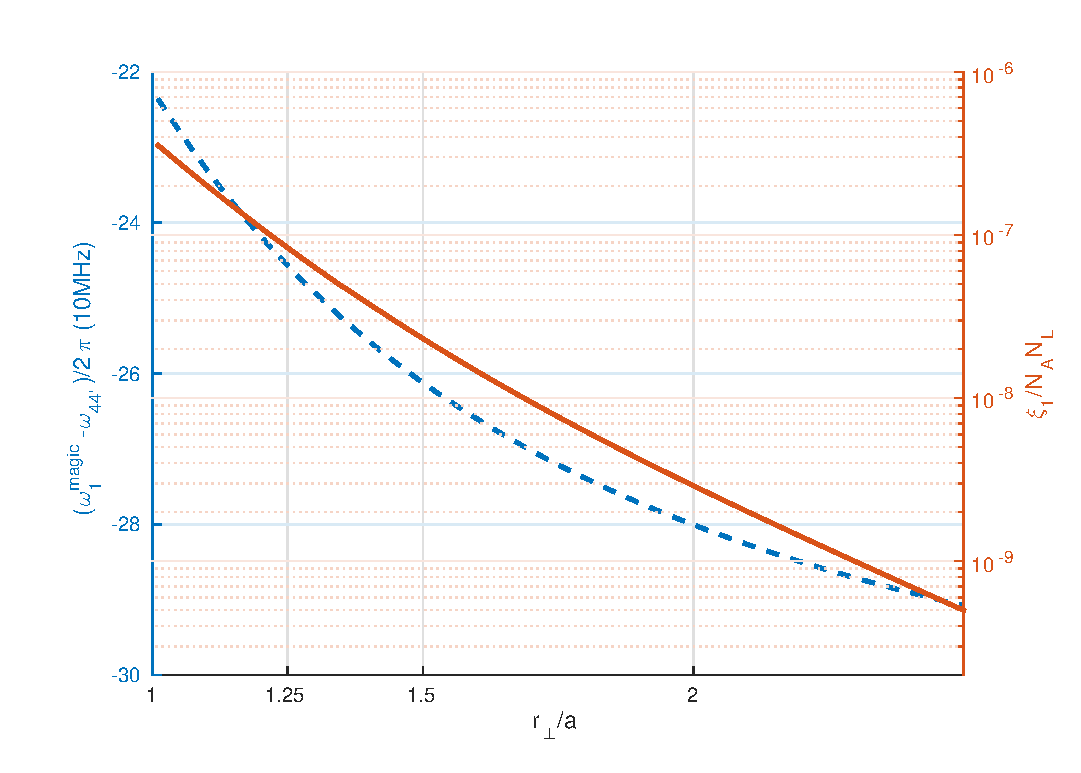
\includegraphics[scale=0.65]{../media/Figs/MagicwavelengSqueezingpara1}}
\end{minipage}
\par\medskip
\begin{minipage}{.91\linewidth}
\centering
\subfloat[]{\label{MagicwavelengSqueezingpara2}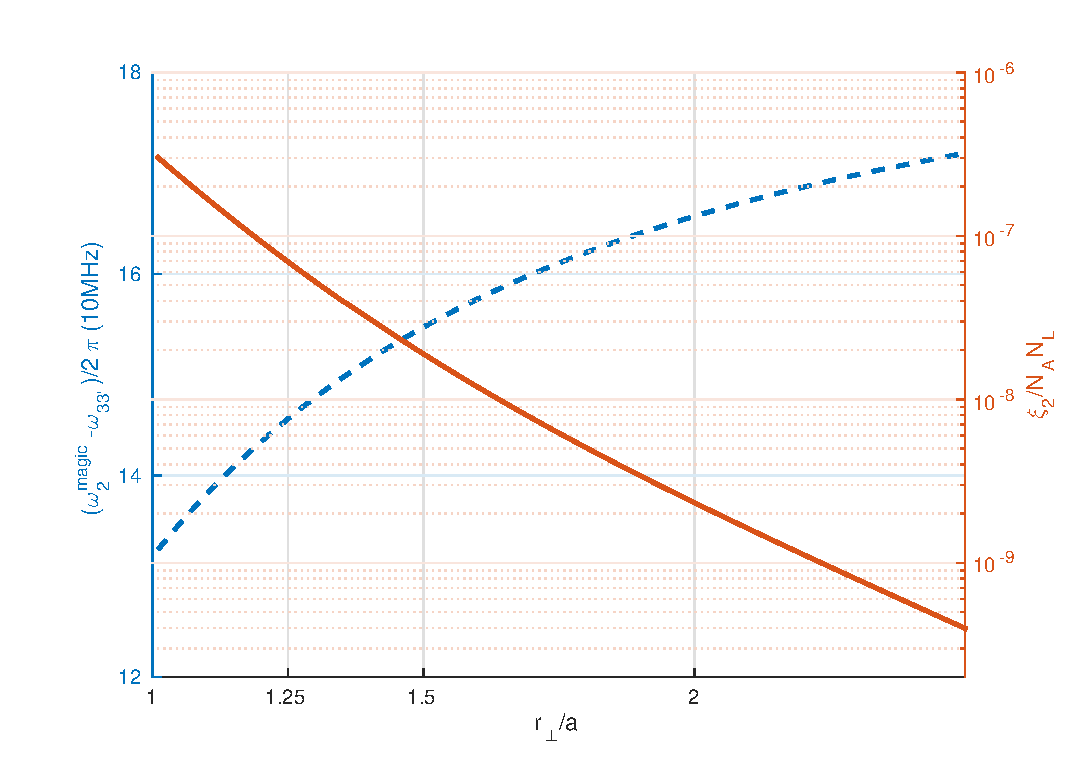
\includegraphics[scale=0.65]{../media/Figs/MagicwavelengSqueezingpara2}}
\end{minipage}
\caption{The magic frequencies (left axis and dashed lines) and corresponding squeezing parameters 
(right axis and solid lines) close to the $ 
F=3\rightarrow F'=3 $ and $ F=4\rightarrow F'=4 $ transition lines. The squeezing parameters are 
calculated for per photon per atom squeezing. }\label{fig:MagicwavelengSqueezingpara}
\end{figure}

\begin{figure}
\begin{minipage}{.91\linewidth}
\centering
\subfloat[]{\label{squeezingparaTerm3_total}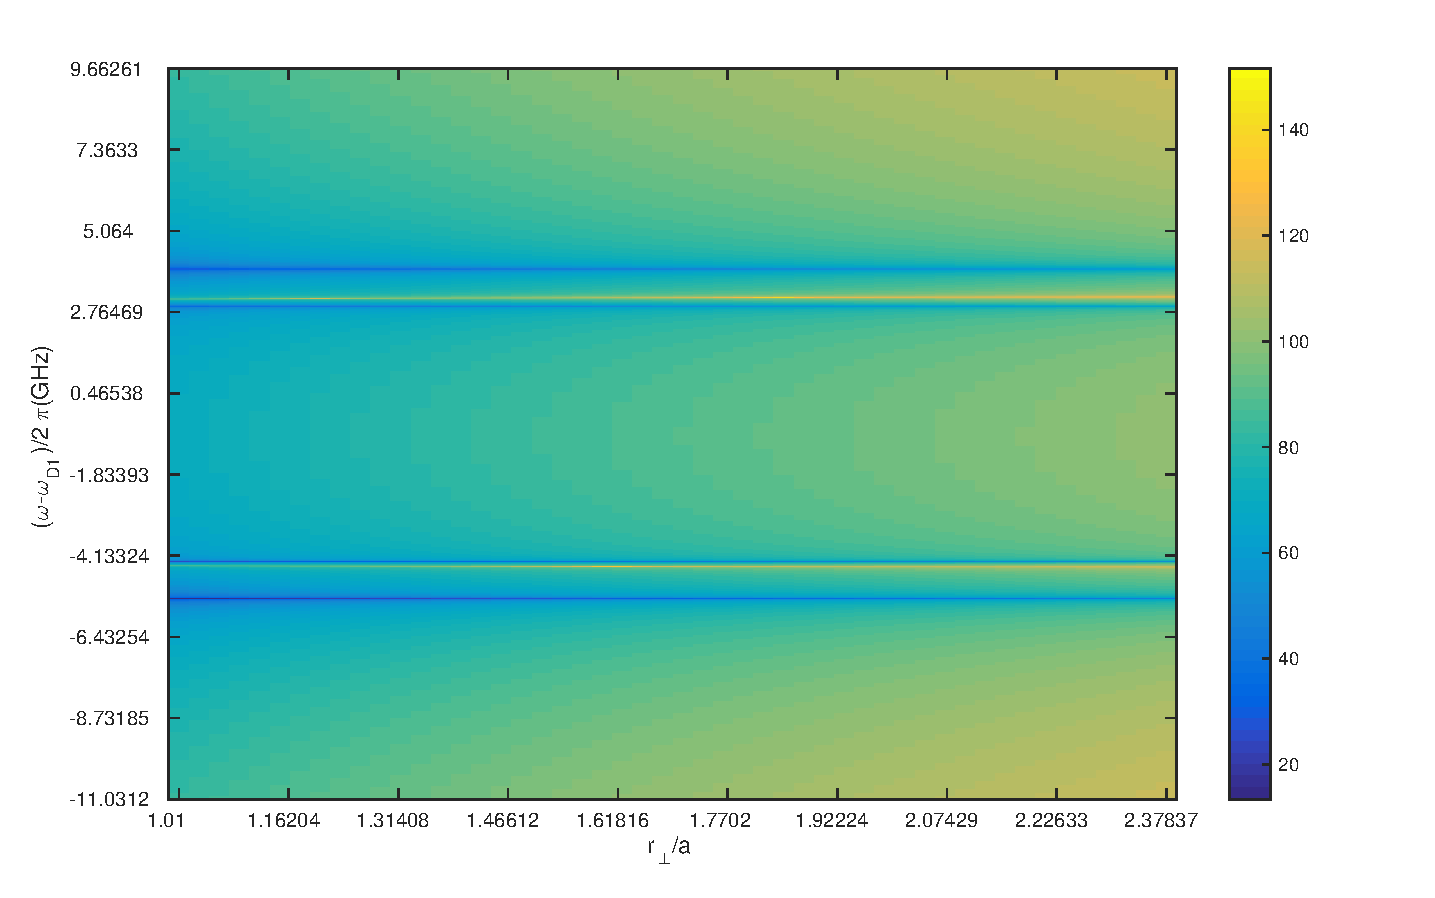
\includegraphics[scale=0.55]{../media/Figs/squeezingparaTerm3_total}}
\end{minipage}
\par\medskip
\begin{minipage}{.91\linewidth}
\centering
\subfloat[]{\label{squeezingparaTerm4_total}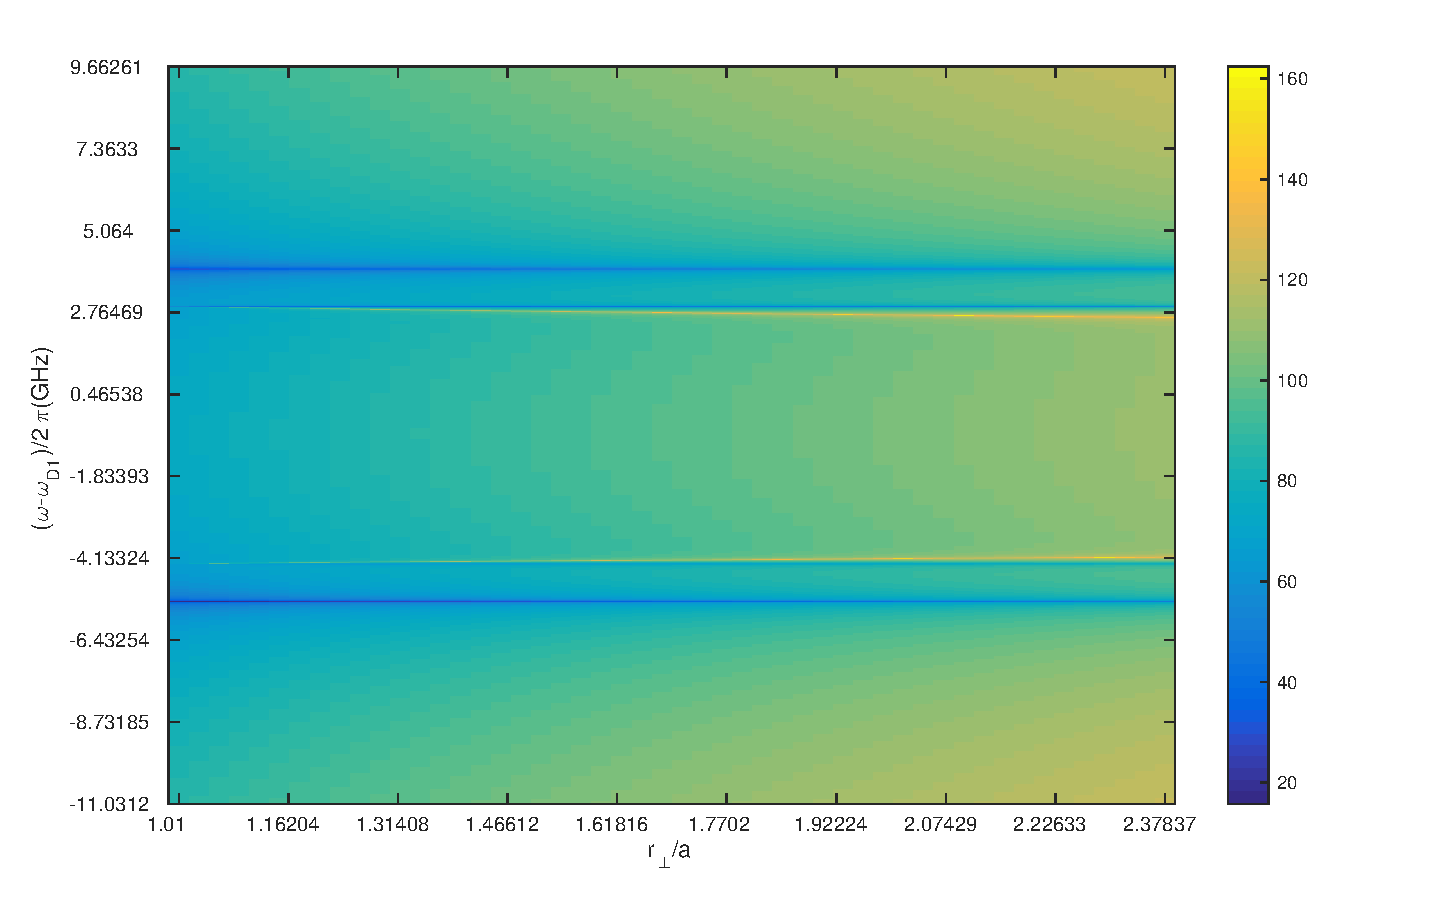
\includegraphics[scale=0.55]{../media/Figs/squeezingparaTerm4_total}}
\end{minipage}
\caption{Squeezing parameters associated to the third and forth terms of the Hamiltonian. The 
colormap shows the value of $ -10\log_{10}(\xi/N_LN_A) $.  All atomic polarizability components are 
included. }
\label{fig:squeezingparaTerms_total}
\end{figure}

\begin{figure}
\begin{minipage}{.91\linewidth}
\centering
{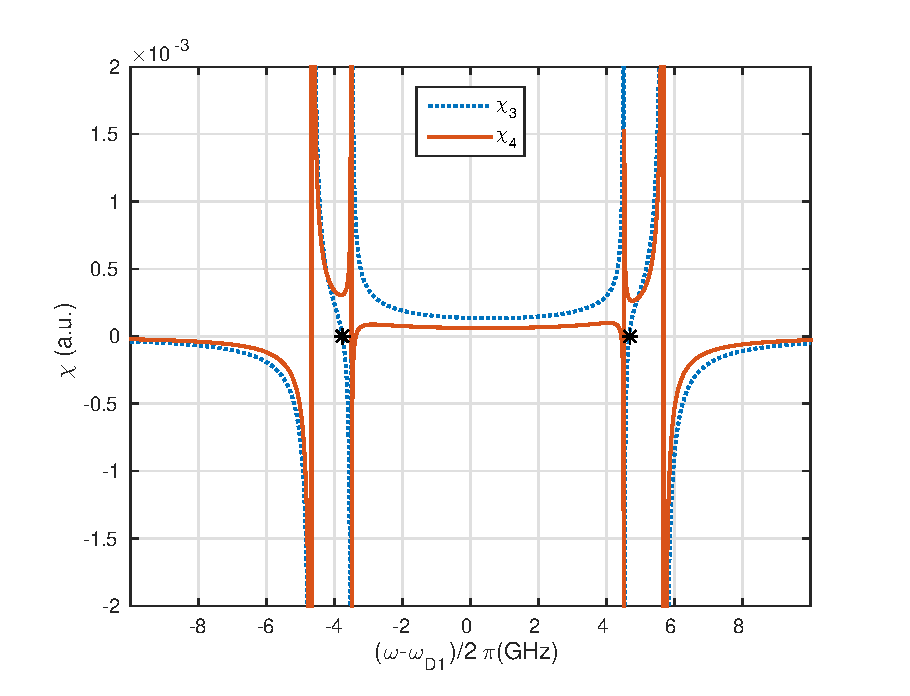
\includegraphics[scale=0.75]{../media/Figs/chi34_total}}
\end{minipage}
\caption{The coupling strengths for the third ($ \chi_3 $) and forth ($ \chi_4 $) terms of the Hamiltonian 
expressed in Equ.~\eqref{eq:JScoupling} for the $ D_1 $ line transitions associated with the clock states. 
All atomic polarizability components are included. The stars indicate where the magic frequencies are 
located.} 
\label{fig:chi34_total}
\end{figure}
